\documentclass[tikz, crop, border=5pt]{standalone}

\usepackage{xcolor}
\usepackage{mathtools}

\DeclareMathOperator{\uniform}{\mathcal{U}}

\usetikzlibrary{
    positioning,
    arrows.meta
}

\tikzset{%
    random variable/.style={%
        circle,
        draw,
        inner sep = 0pt,
        outer sep = 0pt,
        minimum width=1cm
    },
    state/.style={%
        circle,
        draw,
        inner sep = 0pt,
        outer sep = 0pt,
        minimum width=1cm,
        fill=black!20
    },
    observed rv/.style={%
        random variable,
        fill=blue!20,
    },
    unobserved rv/.style={%
        random variable,
        fill=white,
    },
    arrow/.style={%
        >={Stealth[round]},
    },
    formula/.style={%
        rectangle,
        draw=gray,
        rounded corners=2pt,
        inner sep = 2pt,
        outer sep = 0pt,
        minimum width=12cm,
        minimum height=1cm,
    },
}

\begin{document}
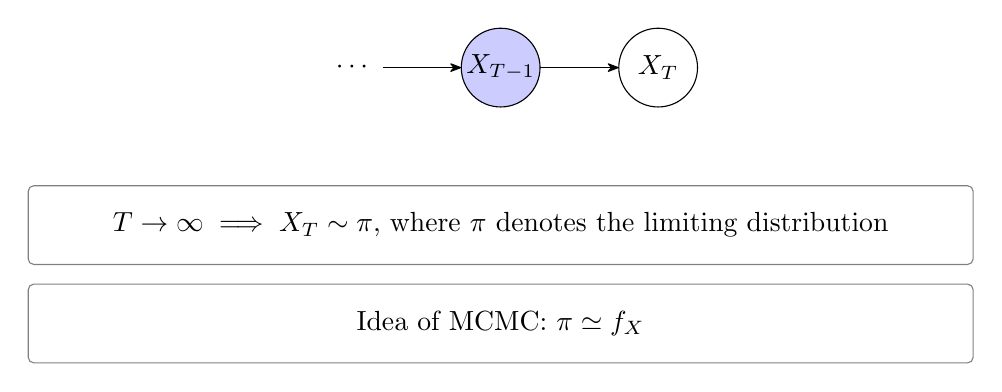
\begin{tikzpicture}

    \node (dots2) {$\cdots$};

    \node[observed rv, right=of dots2] (XT-1) {$X_{T-1}$};
    \node[unobserved rv, right=of XT-1] (XT) {$X_{T}$};

    \draw[arrow, ->] (dots2) to (XT-1);
    \draw[arrow, ->] (XT-1) to (XT);


    \node[formula, below=of XT-1] (formula1) {$T \to \infty \implies X_T \sim \pi$, where $\pi$ denotes the limiting distribution};

    \node[formula, below=0.25cm of formula1] (formula2) {Idea of MCMC: $\pi \simeq f_{X}$};
\end{tikzpicture}
\end{document}